\documentclass{jarticle}
\usepackage[dvipdfmx]{graphicx}
\usepackage{here}
\usepackage{listings}

\begin{document}

\title{最終課題}
\author{1029289895 尾崎翔太}
\date{2019/01/28}

\maketitle
\newpage

\section{システム概要}
レンタルビデオ屋のシステムを作った. 役割は課題1と同じだが, 機能は課題1とは大きく変わっている. 機能としてはユーザによる店舗検索と作品検索と履歴閲覧, 店員によるユーザ登録と貸出/返却, 管理者による店員の登録とメディアの登録と店の登録/削除及び店員がどの店で働くか, メディアをどの店に置くかの管理がある.

\section{実体関連図}
\begin{figure}[tp]
\begin{center}
\includegraphics[scale=0.2]{ER_final.png}
\end{center}
\caption{実体関連図}
\label{fig:er}
\end{figure}
実体関連図は図\ref{fig:er}のようになった. 基本的には課題1のものと同じである. しかし, 異なる点もいくつかある.
\begin{description}
\item[パスワードの追加] \leavevmode \\
ユーザと店員の属性に「パスワード」を追加した. これはインタフェースを分けるためにログインする必要があるためである.
\item[関連「借りている」の三項関連化] \leavevmode \\
課題1のものだと同じユーザが同じメディアを二回借りることができなかったので, 
日付や期間に関する情報を属性ではなく実体として三項関連にした.
\item[属性「返した」と「利用可能」の追加] \leavevmode \\
ひとつのメディアが同時に借りられることのないように追加した.
\item[属性「最大数」と「数」の削除] \leavevmode \\
これは「メディア」ではなく「内容」に関する情報であるため, 「置いてある」の属性として不適切であったため削除した.
\item[属性「通勤手段」と「良いところ」の追加] \leavevmode \\
自明でない多値従属性を作るための属性である.
\end{description}

\section{関係スキーマ}
関係スキーマは以下のようになった.
\begin{itemize}
\item ユーザ(\underline{メールアドレス}, ユーザ名, ユーザ住所, ユーザパスワード)
\item メディア(\underline{mid}, 種類, 利用可能)
\item 内容(\underline{題名}, \underline{発売年}, 長さ, 出版社, ジャンル)
\item 店舗(\underline{店舗名}, \underline{店舗住所}, 総所持数)
\item 店員(\underline{eid}, 店員名, 店員パスワード)
\item 付属情報(\underline{通勤手段}, \underline{店の良い所})
\item 借りている(\underline{メールアドレス}, \underline{mid}, 料金, \underline{貸出日}, \underline{返却日}, 返した)
\item 期間(\underline{貸出日}, 貸出期間, \underline{返却日})
\item 置いてある(\underline{mid}, \underline{店舗名}, \underline{店舗住所})
\item 働いている1(\underline{eid}, \underline{店舗名}, \underline{店舗住所}, \underline{通勤手段})
\item 働いている2(\underline{eid}, \underline{店舗名}, \underline{店舗住所}, \underline{店の良い所})
\item 保存されている(\underline{mid}, \underline{題名}, \underline{発売年})
\end{itemize}
課題3のものに第2章で述べた変更点を反映させただけである. 全ての自明でない関数従属性の左辺は超キーであるからBoyce-Codd正規形である. それぞれのデータ例を以下に示す.
\begin{description}
\item[ユーザ(\underline{メールアドレス}, ユーザ名, ユーザ住所, ユーザパスワード)] \leavevmode \\
\begin{verbatim}
mail                 username useraddress userpw
-------------------- -------- ----------- ---------
yamada@example.jp    山田     A市         yamada
takahashi@example.jp 高橋     B市         takahashi
yoshida@example.jp   吉田     C市         yoshida
baba@example.jp      馬場     D市         baba
hotta@example.jp     堀田     E市         hotta
\end{verbatim}
\item[メディア(\underline{mid}, 種類, 利用可能)] \leavevmode \\
\begin{verbatim}
mid type    available
--- ------- ---------
1   VHS     yes
2   DVD     yes
3   DVD     yes
4   Blu-ray yes
5   Blu-ray yes
\end{verbatim}
\item[内容(\underline{題名}, \underline{発売年}, 長さ, 出版社, ジャンル)] \leavevmode \\
\begin{verbatim}
title published_year length         publisher genre
----- -------------- -------------- --------- -------
ABC   2000           01時間30分00秒 A         movie
ABD   2010           00時間50分30秒 B         drama
ACD   2005           02時間00分00秒 C         variety
BCD   2001           02時間00分00秒 D         anime
BE    2008           02時間10分00秒 E         sport
\end{verbatim}
\item[店舗(\underline{店舗名}, \underline{店舗住所}, 総所持数)] \leavevmode \\
\begin{verbatim}
shopname shopaddress total_media
-------- ----------- -----------
AAA      A市         1
ABD      B市         2
CAD      C市         2
EDC      D市         2
BCD      E市         3
\end{verbatim}
\item[店員(\underline{eid}, 店員名, 店員パスワード)] \leavevmode \\
\begin{verbatim}
eid clerkname clerkpw
--- --------- ---------
1   山田      yamada
2   高橋      takahashi
3   吉田      yoshida
4   馬場      baba
5   堀田      hotta
\end{verbatim}
\item[付属情報(\underline{通勤手段}, \underline{店の良い所})] \leavevmode \\
\begin{verbatim}
commute_method good_point_of_shop
-------------- ------------------
walk           A
walk           B
bicycle        A
bicycle        B
bus            A
\end{verbatim}
\item[借りている(\underline{メールアドレス}, \underline{mid}, 料金, \underline{貸出日}, \underline{返却日}, 返した)] \leavevmode \\
\begin{verbatim}
mail                 mid rental_fee rental_date return_date finished
-------------------- --- ---------- ----------- ----------- --------
yamada@example.jp    1   300        2019/01/04  2019/01/05  yes
takahashi@example.jp 2   300        2019/01/05  2019/01/06  yes
yoshida@example.jp   3   400        2019/01/06  2019/01/08  yes
baba@example.jp      4   400        2019/01/07  2019/01/09  yes
hotta@example.jp     5   500        2019/01/08  2019/01/11  yes
\end{verbatim}
\item[期間(\underline{貸出日}, 貸出期間, \underline{返却日})] \leavevmode \\
\begin{verbatim}
rental_date rental_duration return_date
----------- --------------- -----------
2019/01/04  1日             2019/01/05
2019/01/05  1日             2019/01/06
2019/01/06  2日             2019/01/08
2019/01/07  2日             2019/01/09
2019/01/08  3日             2019/01/11
\end{verbatim}
\item[置いてある(\underline{mid}, \underline{店舗名}, \underline{店舗住所})] \leavevmode \\
\begin{verbatim}
mid shopname shopaddress
--- -------- -----------
1   AAA      A市
2   ABD      B市
3   CAD      C市
4   EDC      D市
5   BCD      E市
\end{verbatim}
\item[働いている1(\underline{eid}, \underline{店舗名}, \underline{店舗住所}, \underline{通勤手段})] \leavevmode \\
\begin{verbatim}
eid shopname shopaddress commute_method
--- -------- ----------- --------------
1   AAA      A市         walk
2   ABD      B市         walk
3   CAD      C市         bicycle
4   EDC      D市         bicycle
5   BCD      E市         bus
\end{verbatim}
\item[働いている2(\underline{eid}, \underline{店舗名}, \underline{店舗住所}, \underline{店の良い所})] \leavevmode \\
\begin{verbatim}
eid shopname shopaddress good_point_of_shop
--- -------- ----------- ------------------
1   AAA      A市         A
2   ABD      B市         B
3   CAD      C市         A
4   EDC      D市         B
5   BCD      E市         A
\end{verbatim}
\item[保存されている(\underline{mid}, \underline{題名}, \underline{発売年})] \leavevmode \\
\begin{verbatim}
mid title published_year
--- ----- --------------
1   ABC   2000
2   ABD   2010
3   ACD   2005
4   BCD   2001
5   BE    2008
\end{verbatim}
\end{description}

\section{機能・インタフェース}
\subsection{ログイン}
\begin{figure}[tp]
\begin{center}
\includegraphics[scale=0.5]{login.png}
\end{center}
\caption{ログイン画面}
\label{fig:login}
\end{figure}
画面は図\ref{fig:login}である. メールアドレスの欄に, ユーザならメールアドレス, 店員ならeid, 管理者なら「supervisor」を入力してパスワードを入力するとログインできる. メールアドレスやeidを用いてuserテーブルやclerkテーブルから対応するパスワードを得て, それが入力されたパスワードと一致するかどうかをチェックしている.

\subsection{ユーザによる店舗検索}
\begin{figure}[tp]
\begin{center}
\includegraphics[scale=0.5]{search.png}
\end{center}
\caption{検索画面}
\label{fig:search}
\end{figure}
\begin{figure}[tp]
\begin{center}
\includegraphics[scale=0.5]{result_shop.png}
\end{center}
\caption{検索結果(店舗)}
\label{fig:result_shop}
\end{figure}
画面は図\ref{fig:search}と図\ref{fig:result_shop}である. 検索は店舗名と住所のAND検索である. 何も入力されていない場合は, その項目に関してはすべて表示される. 入力された店舗名や住所をWHEREの後ろに並べてshopテーブルを検索している. また, 検索結果のソートもできて, これはORDER BYで行っている. 検索で出てきた店舗をクリックすると, その店舗に置いてある作品のリストが表示されるようになっている. 作品をクリックすると詳細情報が見られる.

\subsection{ユーザによる作品検索}
\begin{figure}[tp]
\begin{center}
\includegraphics[scale=0.5]{result_media.png}
\end{center}
\caption{検索結果(作品)}
\label{fig:result_media}
\end{figure}
画面は図\ref{fig:search}と図\ref{fig:result_media}である. 基本的に店舗検索と同じである. mediaテーブルとstoreテーブルとcontentテーブルとputテーブルの四つのテーブルを自然結合したものを検索している. なぜputテーブルを結合しているかというと, 店舗検索からとべる店舗に置いてある作品のリストは, 図\ref{fig:result_media}と同じページであるから, そちらから来た場合に必要になるからである.

\subsection{ユーザによる履歴閲覧}
\begin{figure}[tp]
\begin{center}
\includegraphics[scale=0.5]{history.png}
\end{center}
\caption{履歴画面}
\label{fig:history}
\end{figure}
画面は図\ref{fig:history}である. これはrentテーブルとstoreテーブルを結合したものに対して, このユーザのメールアドレスを用いて検索している.

\subsection{店員によるユーザ登録}
\begin{figure}[tp]
\begin{center}
\includegraphics[scale=0.5]{add_user.png}
\end{center}
\caption{ユーザ登録画面}
\label{fig:add_user}
\end{figure}
画面は図\ref{fig:add_user}である. すべての情報を入力しないとエラーになる. また, メールアドレスも@がなかったり, すでにいるユーザと同じであるとエラーになる. 内部的には, userテーブルにそのメールアドレスの行がないことを確認してから挿入している.

\subsection{店員による貸出/返却}
\begin{figure}[tp]
\begin{center}
\includegraphics[scale=0.5]{rental.png}
\end{center}
\caption{貸出画面}
\label{fig:rental}
\end{figure}
\begin{figure}[tp]
\begin{center}
\includegraphics[scale=0.5]{return.png}
\end{center}
\caption{貸出状況確認画面}
\label{fig:return}
\end{figure}
画面は図\ref{fig:rental}と図\ref{fig:return}である. 貸出については, 空欄や不適切な値に対してエラーを出すようになっている. さらに, userテーブルやmediaテーブル, putテーブルを確認して, ユーザが存在するか, メディアがこの店に置いてあるか, メディアが利用可能かを調べてから, rentテーブルに挿入を行っている. また, このときdurationテーブルにも同時に挿入を行っている. ただし, 挿入しようとしている行が存在しているかどうかを確認して, 存在していない場合だけ挿入するSQL文を実行している. さらに, mediaテーブルのavailableをnoに更新している. 削除については, 図\ref{fig:return}にある「返却する」をクリックすることで行っている. 内部的には, rentテーブルのfinishedをyesに更新している. このとき, 同時にmediaテーブルのavailableもyesに更新している.

\subsection{管理者による店員登録}
\begin{figure}[tp]
\begin{center}
\includegraphics[scale=0.5]{add_clerk.png}
\end{center}
\caption{店員登録画面}
\label{fig:add_clerk}
\end{figure}
画面は図\ref{fig:add_clerk}である. 基本的にはユーザ登録と同じである. ただ, 店員はeidで管理しているので値の重複は起こらない. 一方, 新たなeidを得るために, 現在存在するeidの最大値をclerkテーブルより得て, それに1を加えたものを用いて挿入を行っている.

\subsection{管理者によるメディア登録}
\begin{figure}[tp]
\begin{center}
\includegraphics[scale=0.5]{add_media.png}
\end{center}
\caption{メディア登録画面}
\label{fig:add_media}
\end{figure}
画面は図\ref{fig:add_media}である. 基本的には店員登録と同じである. 異なるのは, mediaテーブルとstoreテーブルとcontentテーブルの3つのテーブルに挿入を行う点である.

\subsection{管理者による店舗登録/削除}
\begin{figure}[tp]
\begin{center}
\includegraphics[scale=0.5]{add_shop.png}
\end{center}
\caption{店舗登録画面}
\label{fig:add_shop}
\end{figure}
\begin{figure}[tp]
\begin{center}
\includegraphics[scale=0.5]{delete_shop.png}
\end{center}
\caption{店舗確認画面}
\label{fig:delete_shop}
\end{figure}
画面は図\ref{fig:add_shop}と図\ref{fig:delete_shop}である. 登録についてはユーザ登録と同じである. 削除については, 返却と同様に「削除」をクリックすることで行っている. ただ, こちらはDELETE文が走るようになっている. また, 同時に実体「店舗」が参加していた関連に対応するテーブルにおいてもDELETE文が走るようになっている. この削除によってどこにも勤めていない店員が現れた場合, 自動的にその店員は削除される.

\subsection{管理者による店員の管理}
\begin{figure}[tp]
\begin{center}
\includegraphics[scale=0.5]{get_clerk.png}
\end{center}
\caption{店員追加画面}
\label{fig:get_clerk}
\end{figure}
\begin{figure}[tp]
\begin{center}
\includegraphics[scale=0.5]{remove_clerk.png}
\end{center}
\caption{店員確認画面}
\label{fig:remove_clerk}
\end{figure}
画面は図\ref{fig:get_clerk}と図\ref{fig:remove_clerk}である. ある店舗における店員の管理が行える. 追加については, 基本的にはユーザ登録と同じである. ただ, 存在しないeidを入力するとエラーを出す. 削除については, 店舗の削除と同様に「削除」をクリックすることで行える. 内部的には, work1テーブルとwork2テーブルにおいて対応する行を削除している. この削除によってどこにも勤めていない店員が現れた場合にもその店員は削除される.

\subsection{管理者によるメディアの管理}
\begin{figure}[tp]
\begin{center}
\includegraphics[scale=0.5]{get_media.png}
\end{center}
\caption{メディア追加画面}
\label{fig:get_media}
\end{figure}
\begin{figure}[tp]
\begin{center}
\includegraphics[scale=0.5]{remove_media.png}
\end{center}
\caption{メディア確認画面}
\label{fig:remove_media}
\end{figure}
画面は図\ref{fig:get_media}と図\ref{fig:remove_media}である. 基本的には店員の管理と同じである. 異なる点は2つある. 1つはこれでどこにも置かれないメディアが現れても, そのメディアは削除されないという点である. もう1つは, メディアの追加/削除に応じてshopテーブルのtotal\_mediaの値を増減させているという点である. これは, 単純にtotal\_mediaの値を得て, それに±1をした値で更新している.


\section{工夫点}
SELECT文以外のSQL文にはPreparedStatementを用いてインジェクション対策をしている. また, 値チェックや同時更新などで一度のアクションで複数回テーブルを触る場合はトランザクションを用いている. ほかには, 店舗削除に伴う削除や, 店員を店舗から外した場合に起こる削除についてはトリガーを用いている. そのトリガーは以下の通りである.
\begin{verbatim}
CREATE TRIGGER deleteshop DELETE ON shop
  BEGIN
    DELETE FROM put WHERE shopname = old.shopname and shopaddress = old.shopaddress;
    DELETE FROM work1 WHERE shopname = old.shopname and shopaddress = old.shopaddress;
    DELETE FROM work2 WHERE shopname = old.shopname and shopaddress = old.shopaddress;
  END;
CREATE TRIGGER deletework AFTER DELETE ON work1
  BEGIN
    DELETE FROM clerk WHERE (SELECT count(*) FROM work1 WHERE clerk.eid = work1.eid) = 0;
  END;
\end{verbatim}
データベース以外の点では, 一部ではあるけれどもソートやフィルターをできるようにしたり, 前のページに戻るをクリックしたときに, 検索やソートの状態を残すようにしたりした.

\section{感想}
いろいろと難しかったと思った. データベースを設計するのも勿論初めてだったが, Webアプリケーションを作ったのも初めてで手間取った. 最終的にできたのを見ると, 同じようなページがいくつもできたので, そのあたりを上手くまとめて記述できればもっと楽だったのだろうと思った. ほかには, 制約の付け方は難しいと思った. 例えば, 「店舗」の「働いている」への参加制約はシステムの方では実現できていない. これは, 直感的には従業員のいない店舗は存在しないが, 実際にシステムで扱う際には誰が働くかということを決めずに, まず店舗を作成したくなるからである. このあたりはどうすれば良いのかなと思った. 授業全体で言うと, 自明でない関数従属性や多値従属性を作りたいものに自然に落とし込むことは困難だと思った. 僕のシステムでも, 貸出日と貸出期間と返却日で関数従属性を作ったが, 数学的に従属しているので, 本当は貸出期間は必要ない. これを用いて正規形するという点でも, それをするために課題1の時点では「借りている」の属性としてこれらを使用しており, 結果として, 同じ人が同じメディアを複数回借りることができなくなっている. 最後に, データベースは本当に様々なところに現れるので, データベースをプログラムから操作することを学べたことは今後に活きてくると思うので, とても有意義な実験だったと思った.


\end{document}
